\documentclass[conference]{IEEEtran}

\IEEEoverridecommandlockouts

\usepackage{amsmath,amssymb,amsfonts, bbold}
\usepackage{cite, hyperref}
\usepackage{algorithm, algpseudocode}
\usepackage{graphicx, multirow, hhline, pgfplots}
\pgfplotsset{compat=1.18}
\usepackage{comment}

\makeatletter

\newcommand{\newlineauthors}{%
\end{@IEEEauthorhalign}\hfill\mbox{}\par
\mbox{}\begin{@IEEEauthorhalign}}  

\def\hlinewd#1{%
\noalign{\ifnum0=`}\fi\hrule \@height #1 %
\futurelet\reserved@a\@xhline}

\makeatother

\begin{document}

\title{Adaptive Kriging Particle Filter and its Application to Terrain-Aided Navigation}

\author{
    \IEEEauthorblockN{HUBERT Bastien}
    \IEEEauthorblockA{\textit{DTIS, ONERA, Université Paris-Saclay} \\
    Palaiseau, France \\
    bastien.hubert@onera.fr}
\and
    \IEEEauthorblockN{DAHIA Karim}
    \IEEEauthorblockA{\textit{DTIS, ONERA, Université Paris-Saclay} \\
    Palaiseau, France \\
    karim.dahia@onera.fr}
\newlineauthors
\and
    \IEEEauthorblockN{MERLINGE Nicolas}
    \IEEEauthorblockA{\textit{DTIS, ONERA, Université Paris-Saclay} \\
    Palaiseau, France \\
    nicolas.merlinge@onera.fr}
\and
    \IEEEauthorblockN{GIREMUS Audrey}
    \IEEEauthorblockA{\textit{IMS, Université de Bordeaux, CNRS, Bordeaux INP} \\
    Talence, France \\
    audrey.giremus@u-bordeaux.fr}
}

\maketitle

\begin{abstract}
In GNSS-denied and poorly-known environments, reliable autonomous navigation is a major challenge, as conventional data fusion algorithms require an extensive knowledge of their surroundings to accurately estimate the vehicle state. To address this issue, we propose to use an adaptive Gaussian process regression to model an approximation of the environment solely based on scarce and noisy samples.

This paper takes advantage of the flexibility of Gaussian processes to dynamically model the underlying terrain by adapting the process to the relevant data at each step. To this end, we propose to locally fit the Gaussian process and perform regression by using only a subset of data points selected according to a proximity criterion. The developed method employs a regularised particle filter to effectively estimate the system state using the output of the regression. By integrating Gaussian process-based terrain predictions, the particle filter can effectively compensate for the lack of precise terrain information, thus enhancing navigation performance in GNSS-denied scenarios.

To evaluate the effectiveness of the proposed approach, simulations were performed in terrain-aided navigation of an unmanned aerial vehicle. Comparative analysis with existing navigation methods illustrates the superiority of the proposed approach in terms of accuracy and robustness.
\end{abstract}

\section{Introduction}

Robust navigation algorithms are a key factor in ensuring an unmanned aerial vehicle (UAV) successfully accomplishes its mission. UAV navigation is generally based on an Inertial Measurement Unit (IMU), which provides a proprioceptive estimate of the vehicle trajectory, but drifts over time. In order to limit the impact of this drift, data fusion algorithms using aiding sensors, like Global Navigation Satellite System (GNSS), must be added to the navigation chain. However, when GNSS data is unavailable, Terrain-Aided Navigation (TAN) \cite{bib:TAN1} \cite{bib:TAN2} \cite{bib:TAN3} is an excellent alternative as a complementary source of information.

TAN consists in estimating the kinematic state of the UAV (\textit{i.e.} its position and velocity) by correlating punctual height measurements to an embedded map, such as a geo-referenced terrain elevation map. However, it is usually impossible to embed an exhaustive knowledge of the overflown terrain on large areas, so TAN is often restricted to small areas, or exploits larger but poorly resolved maps. Moreover, the map sampling is prone to prior mapping errors, so it can be noisy.

This paper addresses the general problem where a UAV embeds a noisy and scarcely sampled geo-referenced map in order to estimate the Posterior Density Function (PDF) of its state. When both the state evolution process and the observation model are linear and degraded by Gaussian white noises, the Kalman Filter (KF) is the estimator that minimises the Mean Squared Integrated Error (MISE). However, in TAN, the measurement function is often highly non-linear, and the initial uncertainty can be so high that the analytical solution provided by an extended KF cannot be used. In such situations, stochastic methods like Particle Filters (PF) are preferred, as they are able to deal with non-linear and ambiguous measurement models.

We propose to use Gaussian Process Regression (GPR), also known as kriging, to locally interpolate the measurement function around the UAV based on the prior knowledge of sparse and noisy punctual data. Gaussian processes have been used in a wide variety of problems including filtering \cite{bib:GP1} \cite{bib:GP2} \cite{bib:GP3}, and, when coupled with estimation methods, they are able capture complex correlations between data and have the interesting property of providing uncertainty measures. This paper presents a new particle filter, the Adaptive Kriging Regularised Particle Filter (AK-RPF), which combines PF with GPR methods to address navigation in poorly-known environments, and demonstrates its capabilities in TAN.

Section II gives a mathematical formulation of the considered problem, while section III presents the AK-RPF. Section IV focuses on the application to TAN and discusses the obtained results. Finally, section V concludes the paper.

\section{Problem Statement}

\subsection{Bayesian Estimation}

The filtering problem can described as such: a system evolves at discrete time step $k$ according to a recursive dynamical process $\mathcal{F}_k : \mathbb{R}^{d_x} \times \mathbb{R}^{d_\nu} \to \mathbb{R}^{d_x}$, and its current state $x_k$ can be indirectly observed through a measurement function $\mathcal{H}_k : \mathbb{R}^{d_x} \to \mathbb{R}^{d_z}$. These functions are degraded by two random noises $\nu_k$ and $\eta_k$ to account for process and measurement uncertainty respectively:

\begin{equation}
\left\{
\begin{aligned}
x_k & = \mathcal{F}_k(x_{k-1}, \nu_k) \\
z_k & = \mathcal{H}_k(x_k) + \eta_k
\end{aligned}
\right. \label{eq:process measure}
\end{equation}
where the measurement noise $\eta_k$ is assumed to be an additive Gaussian white noise of known covariance matrix $R_k$.

The Bayesian paradigm for the filtering problem is to find the PDF of the state at a given time $k$ knowing the initial state $x_0$ and the value of $z_{1:k} = \{z_1 \cdots, z_k\}$, in order to compute the expected state of the system \footnote{It should be noted that alternative estimators, such as the Maximum A Posteriori, could be considered.} at $k$:
\begin{equation}
\hat x_k \triangleq \mathbb{E}(x_k|z_{1:k}) = \int x_k \: p(x_k|z_{1:k}) \: dx_k \label{eq:expectation}
\end{equation}
and the associated error covariance matrix:
\begin{equation}
P_k \triangleq \mathbb{V}(\hat{x}_k) = \int (x_k - \hat{x}_k)(x_k - \hat{x}_k)^T p(x_k|z_{1:k}) dx_k
\end{equation}

In principle, the PDF may be recursively computed in two steps:
\begin{itemize}
\item The prediction step, which consists of computing the prior density function with the Chapman-Kolmogorov equation:
\end{itemize}
\begin{equation}
p(x_k|z_{1:k-1}) = \int p(x_k|x_{k-1}) \: p(x_{k-1}|z_{1:k-1}) \: dx_{k-1}
\end{equation}
\begin{itemize}
\item The correction step, whose goal is to update the PDF from Bayes' theorem:
\end{itemize}
\begin{equation}
p(x_k|z_{1:k}) = \frac{p(z_k|x_k) \: p(x_k|z_{1:k-1})}{\int p(z_k|x_k) \: p(x_k|z_{1:k-1}) \: dx_k} \label{eq:correction}
\end{equation}

If both the dynamical process and the measurement function in (\ref{eq:process measure}) are linear and the noises are Gaussian, the estimation problem can be solved analytically by the Kalman filter \cite{bib:Ristic}. However, in severely non-linear cases, the highly restrictive assumptions required by the Kalman equations are not met, and stochastic methods are thus used instead. Particle filtering has long been considered for that purpose, and proven to be efficient in highly multimodal scenarios. Two particle filters will be presented in this article: the Regularised Particle Filter (RPF) \cite{bib:RPF} and the Adaptive Kriging Regularised Particle Filter (AK-RPF). The RPF is a state of the art algorithm that uses kernel density estimation to propose a better estimation of the PDF than the standard PF, while the AK-RPF is the contribution of this paper. It extends the RPF by reconstructing the measurement function from noisy and partially sampled data. However, it should be noted that it could leverage any type of particle filter.

\subsection{Regularised Particle Filter}

Particle Filters \cite{bib:tutorial} are a class of algorithms using importance sampling methods to compute an approximation of (\ref{eq:expectation}). Standard PFs usually approximate the PDF by a mixture of Dirac distributions:
\begin{equation}
p(x_k|z_{1:k}) \approx \sum_{i=1}^{N_p} w_k^i \: \delta\left(x_k - x_k^i\right) \label{eq:PDF}
\end{equation}
where $\delta$ denotes the Dirac distribution, $\{x_k^i, i \in [\![1, N_p]\!]\}$ are $N_p$ elements of $\mathbb{R}^{d_x}$, called particles, drawn at each iteration, and $\{w_k^i, i \in [\![1, N_p]\!]\}$ are their respective weights, positive scalars summing to unity.  If the state evolution is Markovian and the particles are propagated according to (\ref{eq:process measure}), a recursive relation between the weights can be established:
\begin{equation}
w_k^i \propto w_{k-1}^i \: p\left(z_k|x_k^i\right)\label{eq:w recursive}
\end{equation}

It can be proven \cite{bib:weight variance} that the variance of the weights can only increase over time, so an additional resampling step can be necessary if the effective sample size is inferior to a threshold:
\begin{equation}
\frac{1}{\sum_{i=1}^{N_p}\left(w_k^i\right)^2} <  \alpha_{th} \: N_p \label{eq:resampling}
\end{equation}
with $\alpha_{th} \in [0, 1]$ a parameter of the filter.

However, repeated resampling can lead to particle impoverishment, which the RPF prevents. In the case of RPF, the PDF (\ref{eq:PDF}) is being smoothed by using kernels instead of Dirac distributions:
\begin{equation}
p(x_k|z_{1:k}) \approx \sum_{i=1}^{N_p} w_k^i \: \mathcal{K}_h\left(x_k - x_k^i\right)
\end{equation}
where $\mathcal{K}_h$ is the scaled kernel of dilatation factor $h$ associated with a kernel $\mathcal{K}$:
\begin{equation}
\mathcal{K}_h : x \mapsto \frac{1}{h^{d_x}} \mathcal{K}\left(\frac{x}{h}\right)
\end{equation}
and is also a kernel.

Under the assumptions that all the particles have the exact same weights (which is the case after resampling) and that $p$ is Gaussian of unit variance, the non-scaled kernel that minimises the MISE is the Epanechnikov kernel \cite{bib:Epanechnikov}:
\begin{equation}
\mathcal{K} : x \mapsto \frac{d_x+2}{2c_{d_x}}\left(1-||x||_2^2\right) \: \mathbb{1}_{\{||\cdot||_2\leq1\}}(x) \label{eq:Epanechnikov}
\end{equation}
and the associated optimal dilatation factor is:
\begin{equation}
h_{opt} = \alpha_{reg}\left(\frac{8}{c_{d_x}} \: (d_x+4) \left(2\sqrt{\pi}\right)^{d_x}\right)^{\frac{1}{d_x+4}} \: N_p^{-\frac{1}{d+4}} \label{eq:h opt}
\end{equation}
where $\alpha_{reg} \in [0,1]$ is a modulation factor introduced to avoid over-smoothing the PDF when the Gaussian assumption is not verified. Unit variance can be achieved by whitening (\textit{i.e.} multiplying by a square root of its covariance matrix) each particle.

Algorithm \ref{alg:RPF} gives the pseudo-code corresponding to the sequential implementation of the RPF.

\begin{algorithm}[ht]
\begin{algorithmic}
\For{$i \in [\![1, N_p]\!]$}
\State Draw $x_k^i$ from $p(\cdot|x_{k-1}^i)$ \Comment{Prediction}
\State Compute $w_k^i$ according to (\ref{eq:w recursive}) \Comment{Correction}
\EndFor
\State $s \gets \sum_{i=1}^{N_p} w_k^i$
\For{$i \in [\![1, N_p]\!]$}
\State $w_k^i \gets w_k^i / s$ \Comment{Normalisation}
\EndFor
\State $\hat x_k \gets \sum_{i=1}^{N_p} w_k^i x_k^i$ \Comment{Estimation}
\State $\hat P_k \gets \sum_{i=1}^{N_p} w_k^i (x_k^i - \hat x_k) (x_k^i - \hat x_k)^T$
\If{(\ref{eq:resampling})}
\State $\text{Resampling}\left(x_k^{1:N_p},w_k^{1:N_p}\right)$ \Comment{Resampling}
\For{$i \in [\![1, N_p]\!]$}
\State Draw $\varepsilon_k^i$ from (\ref{eq:Epanechnikov}) \Comment{Regularisation}
\State Compute $h_{opt}$ from (\ref{eq:h opt})
\State $x_k^i \gets x_k^i + h_{opt}\:\hat P_k^{\frac{1}{2}}\:\varepsilon_k^i$
\EndFor
\State $\hat x_k \gets \sum_{i=1}^{N_p} w_k^i x_k^i$ \Comment{Re-estimation}
\State $\hat P_k \gets \sum_{i=1}^{N_p} w_k^i (x_k^i - \hat x_k) (x_k^i - \hat x_k)^T$
\EndIf
\end{algorithmic} \caption{RPF} \label{alg:RPF}
\end{algorithm}

\section{Adaptive Kriging Particle Filter}

\subsection{Navigation in Poorly-Known Environment}

In usual GNSS-denied data fusion scenarios, the system embeds a precise map of its environment (for example, an elevation map for TAN), and is thus able to evaluate the measurement function at any point. This is required in the correction step (\ref{eq:correction}) of Bayesian filtering, in which the measurement function is used to compute the likelihood:
\begin{equation}
p(z_k|x_k^i) \propto \text{exp}\left(-\frac{1}{2}{y_k^i}^T\:R_k^{-1}\:y_k^i\right) \label{eq:likelihood}
\end{equation}
where
\begin{equation}
y_k^i \triangleq z_k - \mathcal{H}_k(x_k^i) \sim \mathcal{N}(0, R_k) \label{eq:innovation}
\end{equation}
is the innovation term associated with particle $x_k^i$, and follows the law of $\eta_k$.

However, if the system only has access to sparse data (\textit{e.g.} from a previous reconnaissance mission), a simple bilinear interpolation of the map is likely to yield poor results. What is more, the uncertainty of the interpolation will be unknown, so the filter might be overconfident in the reconstructed map, and fail to converge. Figure \ref{fig:interpolation} illustrates the situation.

\begin{figure}[ht]
\centerline{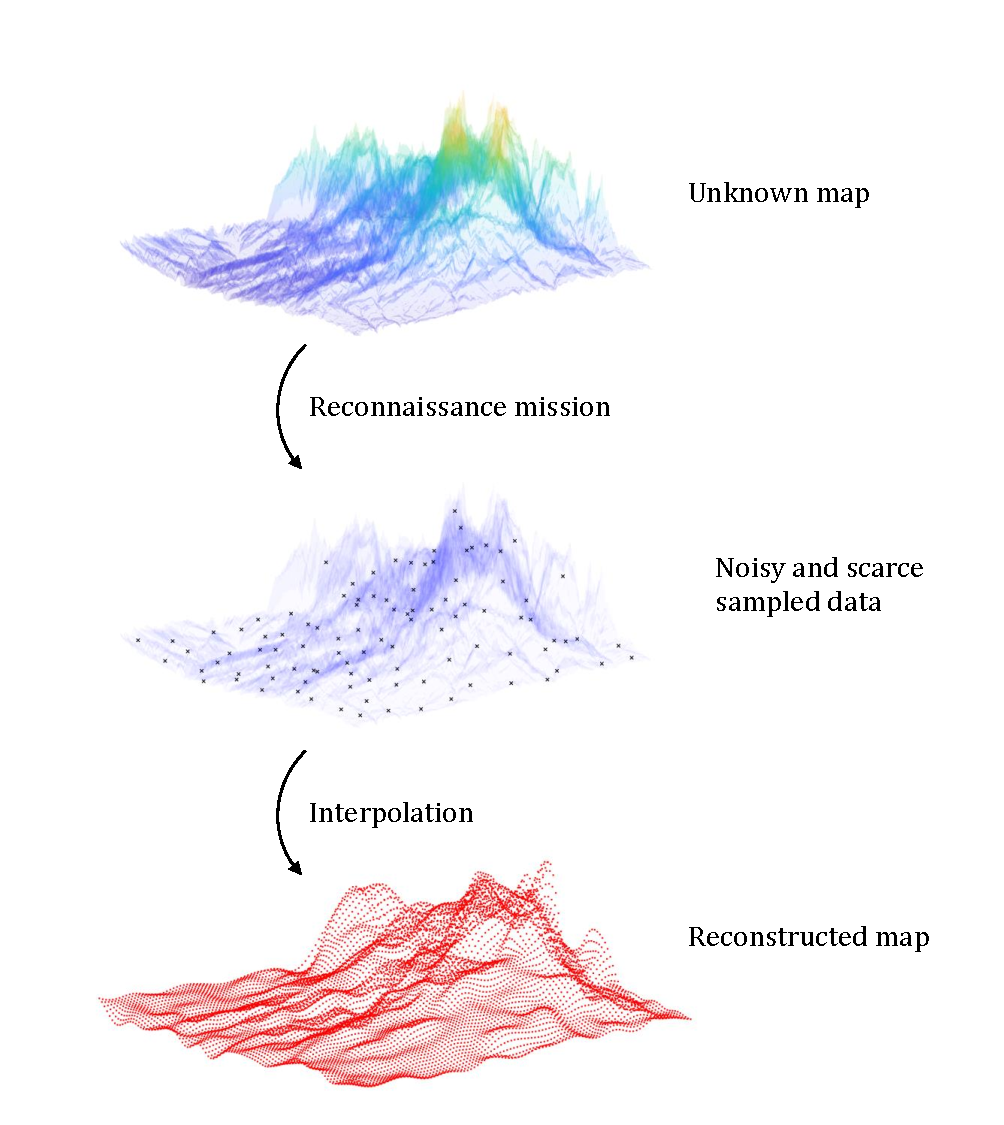
\includegraphics[width=7cm]{interpolation.pdf}}
\caption{Steps to reconstructing the unknown map by interpolating scarce data sampled during a reconnaissance mission prior to the current mission} \label{fig:interpolation}
\end{figure}

\subsection{Gaussian Process Regression}

In order to address both of these issues, we propose to use Gaussian Processes Regression (GPR), an analytical interpolation technique that has the advantage of giving an estimation of the precision of the interpolation in the form of a covariance matrix at each interpolated point. Performing a GPR on the sampled data will give a better estimate of $\mathcal{H}_k$ in points where it wasn't sampled than a bilinear interpolation would, and provide the associated uncertainty of the estimation.

A Gaussian Process (GP) is a stochastic process such that every sub-collection of its samples follows a Gaussian distribution. It is written as such:
\begin{equation}
\mathcal{H}(\cdot) \sim \mathcal{GP}( \mu(\cdot), \mathcal{K}(\cdot, \cdot))
\end{equation} \label{eq:GP}
where $\mu$ is the mean function of the GP, and $k$ is its covariance function.

For the sake of simplicity, when considering random variables $x \triangleq [x^1, \: \cdots, \: x^{\tilde n}]^T$ and $\tilde{x} \triangleq [\tilde x^1, \: \cdots, \: \tilde x^{\tilde n}]^T$, we will be using the following notations:
\begin{equation}
\mathcal{K}(x, \tilde{x}) = \begin{bmatrix}
\mathcal{K}(x^1, \tilde x^1) & \cdots & \mathcal{K}(x^1, \tilde x^{\tilde n}) \\
\vdots & \ddots & \vdots \\
\mathcal{K}(x^n, \tilde x^1) & \cdots & \mathcal{K}(x^n, \tilde x^{\tilde n})
\end{bmatrix}
\end{equation}
\begin{equation}
\mu(x) = [\mu(x^1), \: \cdots, \: \mu(x^n)]^T
\end{equation}

Consider $h = \mathcal{H}(x)$ and $\tilde{h} = \mathcal{H}(\tilde{x})$ two vectors of random variables, we wish to infer the values of $h$ using the prior knowledge of $\tilde{h}$. However, the two vectors are not directly available, but are degraded by two Gaussian white noises to model sensor uncertainty:
\begin{equation}
\left\{
\begin{matrix}
\forall i \in [\![1, n]\!], & z^i \triangleq \mathcal{H}(x^i) + \eta^i & \eta^i \sim(0, R) \\
\forall j \in [\![1, \tilde n]\!], & \tilde z^j \triangleq \mathcal{H}(\tilde x^j) + \tilde\eta^j & \tilde\eta^j \sim(0, \tilde R)
\end{matrix}
\right. \label{eq:noisy H}
\end{equation}
where $\eta^i$ and $\tilde\eta^j$ are independent, and $R$ and $\tilde R$ are two covariance matrices.

From (\ref{eq:noisy H}) and (\ref{eq:GP}), we deduce that the joint distribution of $z \triangleq [z^1, \: \cdots, \: z^{\tilde n}]^T$ and $\tilde{z} \triangleq [\tilde z^1, \: \cdots, \: \tilde z^{\tilde n}]^T$ follows a multivariate Gaussian distribution:
\begin{equation}
\begin{bmatrix}z \\ \tilde{z}\end{bmatrix} \sim \mathcal{N}\left(
\begin{bmatrix}\mu(x) \\ \mu(\tilde{x})\end{bmatrix},
\begin{bmatrix}
\mathcal{K}(       x,  x) + I_n\!\otimes\!R \hspace{-3.5mm} &
\mathcal{K}(       x,  \tilde{x}) \\
\mathcal{K}(x, \tilde{x})^T & \hspace{-3.5mm}
\mathcal{K}(\tilde{x}, \tilde{x}) + I_{\tilde n}\!\otimes\!\tilde R
\end{bmatrix}
\right)
\end{equation}

Thus \cite{bib:Rasmussen}, the conditional distribution $z|\tilde{z}$ follows a Gaussian distribution of mean $\mu^*(x, \tilde{x}, \tilde{z})$ and covariance matrix $R^*(x, \tilde{x})$, with:
\begin{equation}
\left\{
\begin{aligned}
A(x, \tilde{x}) &  \triangleq
\mathcal{K}(x, \tilde{x}) \:
\left(\mathcal{K}(\tilde{x}, \tilde{x}) + I_{\tilde n} \otimes \tilde R\right)^{-1} \\
\mu^*(x, \tilde{x}, \tilde{z}) & \triangleq
\mu(x) + A(x, \tilde{x}) \:
(\tilde{z} - \mu(\tilde{x})) \\
R^*(x, \tilde{x}) & \triangleq
\mathcal{K}(x, x) +
I_n \otimes R -
A(x, \tilde{x}) \:
\mathcal{K}(x, \tilde{x})^T
\end{aligned}
\right. \label{eq:GPR}
\end{equation}

If $\tilde{z}$ represents the noisy prior observations of $\mathcal{H}_k$ corresponding to the input $\tilde{x}$, (\ref{eq:GPR}) can be used to rewrite the measurement function from (\ref{eq:process measure}) as:
\begin{equation}
z_k = \mu^*(x_k, \tilde{x}, \tilde{z}) + \eta^*_k
\end{equation}
with $\eta^*_k$ a Gaussian white noise of variance $R^*(x_k, \tilde{x})$.

Similarly, (\ref{eq:likelihood}) becomes:
\begin{equation}
p(z_k|x_k^i) \propto \text{exp}\left(-\frac{1}{2}{y_k^{*i}}^T\:R^*(x_k, \tilde{x})^{-1}\:y_k^{*i}\right) \label{eq:likelihood GPR}
\end{equation}
with
\begin{equation}
y_k^{*i} \triangleq z_k - \mu^*\left(x_k^i, \tilde{x}, \tilde{z}\right) \sim \mathcal{N}(0, R^*(x_k, \tilde{x}))\label{eq:innovation GPR}
\end{equation}

\subsection{Adaptive Kriging}

When performing the GPR in (\ref{eq:GPR}), it is crucial that the relevant data is used as prior information and the GP correctly fits to the spatial non-stationarity of the terrain to ensure the best possible interpolation. The AK-RPF achieves this by adaptively selecting the samples used for the regression. More precisely, it only considers sampled data inside a moving window centred on the current predicted state:
\begin{equation}
W_k \triangleq \{i \in  [\![1, N_{GP}]\!] : ||\tilde x^i - \pi_g(\hat x_{k|k-1})||_2 < r_k\} \label{eq:fenêtre}
\end{equation}
where $\hat x_{k|k-1} \triangleq \mathbb{E}(x_k|z_{1:k-1}) = \sum_{i=1}^{N_p} w_{k-1}^i x_k^i$ is the predicted state, $W_k$ is the set of indices used to perform the GPR at iteration $k$, $\pi_g$ is the orthogonal projector on the ground, and $r_k$ is the adaptive window radius. The radius (\ref{eq:rayon}) is chosen proportional to the semi-major axis of the $3\sigma$-ellipsoid to ensure that the elevation of most particles will be interpolated instead of extrapolated. To prevent extreme scarcity of data, we also impose that the window must contain at least $N_{W,min}$ points:
\begin{equation}
\left\{
\begin{aligned}
r_k & \triangleq \text{min}\{r \in [r_{min,k}, +\infty[ \:: \text{Card}(W_k) \geq N_{W,min}\} \\
r_{min,k} & \triangleq \alpha_W \times \underset{\lambda \in \text{sp}(\pi_g(P_{k|k-1}))}{\text{max}}\left(3\sqrt{\lambda}\right)
\end{aligned}
\right. \label{eq:rayon}
\end{equation}
where $P_{k|k-1} \triangleq \mathbb{V}(\hat{x}_{k|k-1}) = \sum_{i=1}^{N_p} w_{k-1}^i (x_k^i - \hat x_{k|k-1}) (x_k^i - \hat x_{k|k-1})^T$ is the covariance matrix of $\hat{x}_{k|k-1}$, and $\alpha_W \in \mathbb{R}_+$ and $N_{W,min} \in \mathbb{N}$ are parameters of the filter. The adaptive window also has the advantage of reducing the computational load by reducing the size of the covariance matrices in (\ref{eq:GPR}).

Figure \ref{fig:fenêtre} shows a diagram representing the kriging window and the computation of its radius.

\begin{figure}[ht]
\centerline{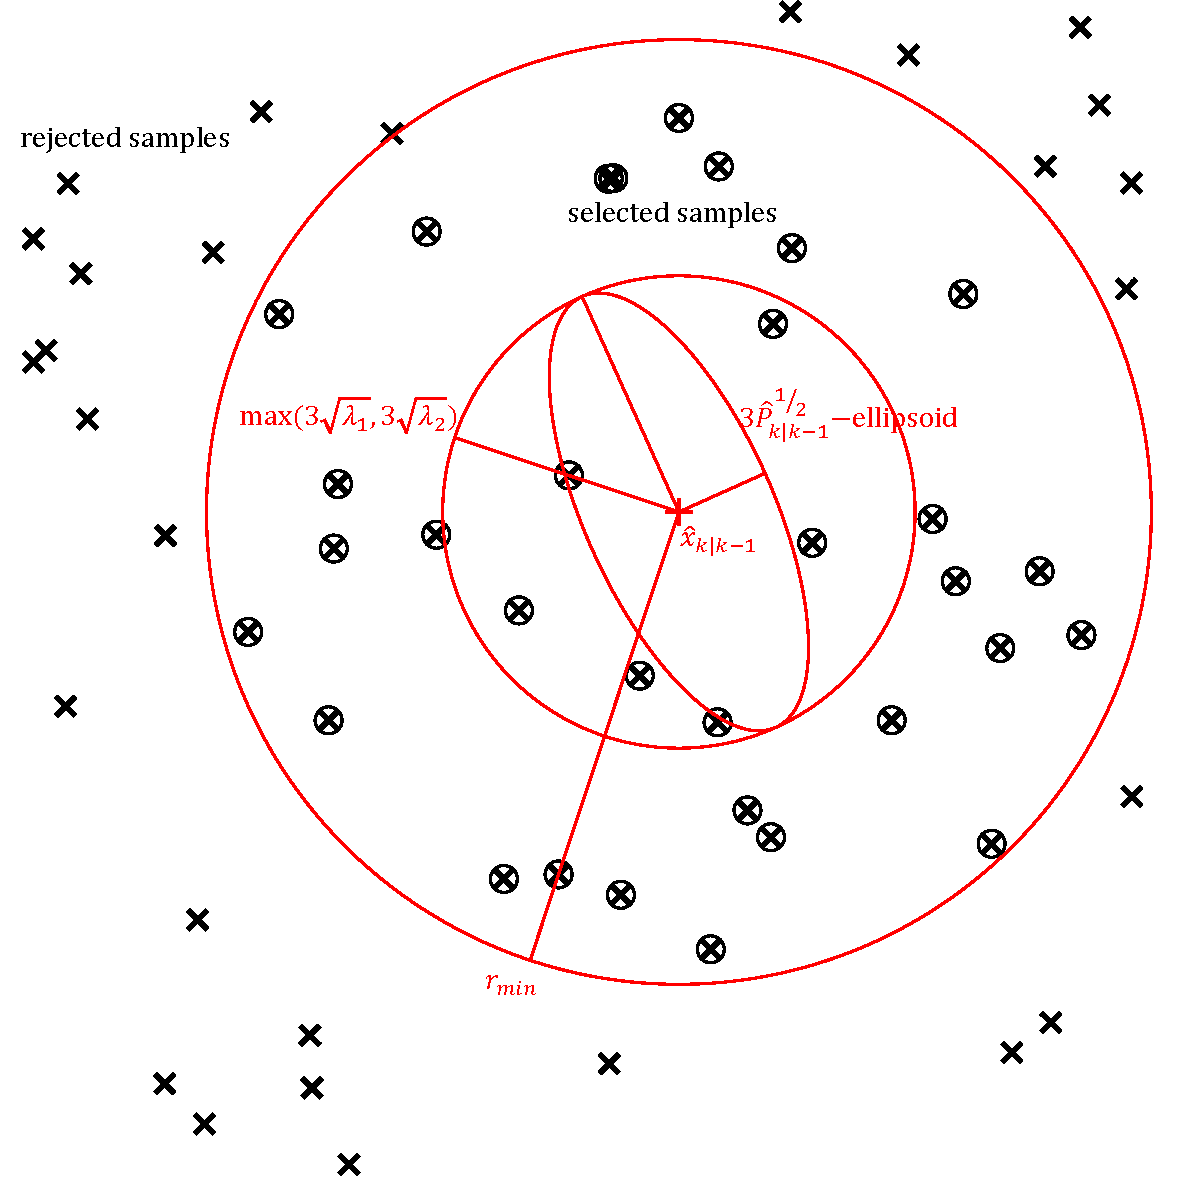
\includegraphics[width=7cm]{fenêtre.pdf}}
\caption{The adaptive kriging window corresponds to the circumcircle of $3\sigma$-ellipsoid of the predicted state enlarged by a factor $\alpha_W$} \label{fig:fenêtre}
\end{figure}

If $(\tilde{x},\tilde{z})$ is the set of the prior data, we can define $\tilde{x}_k$ (resp. $\tilde{z}_k$) as the subset of $\tilde{x}$ (resp. $\tilde{z}$) whose element indices are in $W_k$. To ensure the estimated measurement function given by (\ref{eq:GPR}) fits as closely as possible to the truth, the hyperparameters of the GP are evaluated using Maximum Likelihood Estimation (MLE) on the log-likelihood:
\begin{equation}
\begin{aligned}
l(\theta, \tilde{x}_k, \tilde{z}_k) =
& -\frac{1}{2}
(\tilde{z}_k - \mu_\theta(\tilde{x}_k))^T
\mathcal{K}_\theta(\tilde{x}_k,\tilde{x}_k)^{-1}
(\tilde{z}_k - \mu_\theta(\tilde{x}_k)) \\
& -\frac{1}{2}
\text{log}(\text{det}(\mathcal{K}_\theta(\tilde{x}_k,\tilde{x}_k))) - \frac{n}{2} \text{log}(2 \pi)
\end{aligned} \label{eq:log-likelihood}
\end{equation}
where $l(\theta, z, x) = \text{log}(p_\theta(z|x))$ is the log-likelihood of the GP, and $\theta$ are its concatenated hyperparameters. A gradient descent on (\ref{eq:log-likelihood}) can be performed to iteratively compute $\theta$ until:
\begin{equation}
\text{tr}\left(\left(\alpha_\theta \alpha_\theta^T - \mathcal{K}_\theta(\tilde{x}_k,\tilde{x}_k)^{-1}\right)\frac{\partial \mathcal{K}_\theta}{\partial \theta}(\tilde{x}_k,\tilde{x}_k)\right) = 0 \label{eq:gradient}
\end{equation}
with
\begin{equation}
\alpha_\theta \triangleq \mathcal{K}_\theta(\tilde{x}_k,\tilde{x}_k)^{-1} (\tilde{z}_k - \mu_\theta(\tilde{x}_k))
\end{equation}

The pseudo-code for the AK-RPF is given by Algorithm \ref{alg:AK-RPF}.

\begin{algorithm}
\begin{algorithmic}
\For{$i \in [\![1, N_p]\!]$}
\State Draw $x_k^i$ from $p(\cdot|x_{k-1}^i)$ \Comment{Prediction}
\EndFor
\State Compute $r_k$ from (\ref{eq:rayon}) \Comment{Adaptive selection}
\State Extract $(\tilde{x}_k,\tilde{z}_k)$ from $(\tilde{x},\tilde{z})$ using (\ref{eq:fenêtre})
\State Fit $\theta$ to $(\tilde{x}_k,\tilde{z}_k)$ with (\ref{eq:gradient}) \Comment{Adaptive GP}
\For{$i \in [\![1, N_p]\!]$}
\State Compute $p(z_k|x_k^i)$ according to (\ref{eq:likelihood GPR}) \Comment{Kriging}
\State Compute $w_k^i$ according to (\ref{eq:w recursive}) \Comment{Correction}
\EndFor
\State $s \gets \sum_{i=1}^{N_p} w_k^i$
\For{$i \in [\![1, N_p]\!]$}
\State $w_k^i \gets w_k^i / s$ \Comment{Normalisation}
\EndFor
\State $\hat x_k \gets \sum_{i=1}^{N_p} w_k^i x_k^i$ \Comment{Estimation}
\State $\hat P_k \gets \sum_{i=1}^{N_p} w_k^i (x_k^i - \hat x_k) (x_k^i - \hat x_k)^T$
\If{(\ref{eq:resampling})}
\State $\text{Resampling}\left(x_k^{1:N_p},w_k^{1:N_p}\right)$ \Comment{Resampling}
\For{$i \in [\![1, N_p]\!]$}
\State Draw $\varepsilon_k^i$ from (\ref{eq:Epanechnikov}) \Comment{Regularisation}
\State Compute $D_k$ such that $D_k^T D_k = \hat P_k$
\State Compute $h_{opt}$ from (\ref{eq:h opt})
\State $x_k^i \gets x_k^i + h_{opt}\:D_k\:\varepsilon_k^i$
\EndFor
\State $\hat x_k \gets \sum_{i=1}^{N_p} w_k^i x_k^i$ \Comment{Re-estimation}
\State $\hat P_k \gets \sum_{i=1}^{N_p} w_k^i (x_k^i - \hat x_k) (x_k^i - \hat x_k)^T$
\EndIf
\end{algorithmic} \caption{AK-RPF} \label{alg:AK-RPF}
\end{algorithm}

\section{Application to TAN}

\subsection{Simulation Scenario}

In this paper, we consider a UAV navigating above an uneven terrain in a uniform rectilinear motion. The state is represented by the $d_x = 6$ dimension vector $x$:
\begin{equation}
x = [p_x, \: p_y, \: p_z, \: v_x, \: v_y, \: v_z]^T \label{eq:x}
\end{equation}
with $p_i$ being the $i^{th}$ position coordinate, and $v_i$ being its associated velocity. The precise location at any given time of the UAV is unknown, but a radar altimeter gives access to a noisy estimation of the altitude above the ground, as depicted in Figure \ref{fig:TAN}.

\begin{figure}[ht]
\centerline{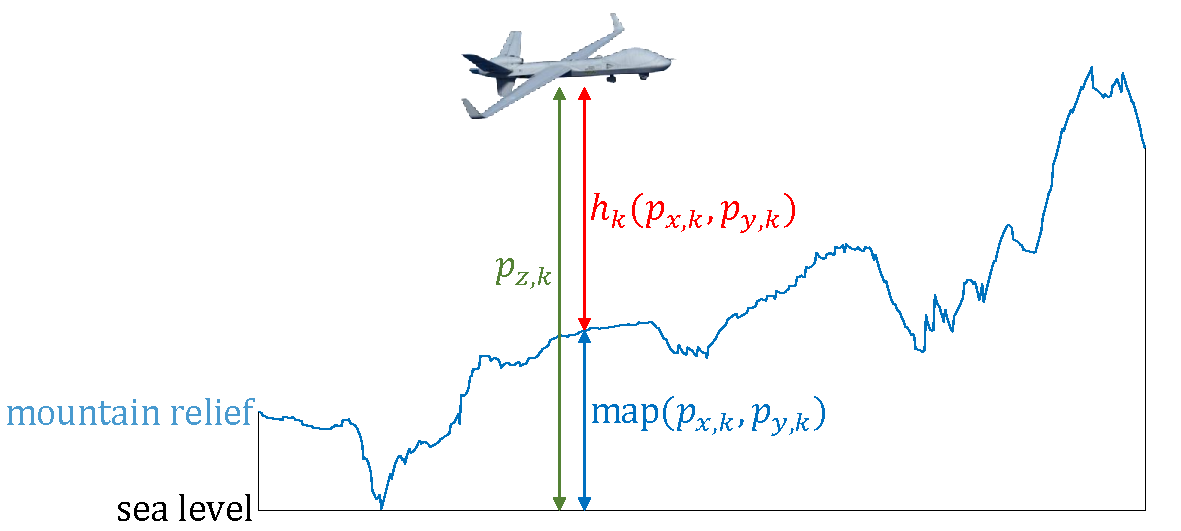
\includegraphics[width=7cm]{TAN.pdf}}
\caption{The TAN measurement model uses a radar altimeter to estimate the distance between the UAV and the ground as the difference between the UAV's vertical position and the elevation of the terrain below} \label{fig:TAN}
\end{figure}

The system from (\ref{eq:process measure}) can thus be written as:
\begin{equation}
\left\{
\begin{aligned}
x_k & = F x_{k-1} + \nu_k \\
z_k & = p_{z, k} - \text{map}(p_{x, k},  p_{y, k}) + \eta_k
\end{aligned}
\right.
\end{equation}
with $\nu_k \sim \mathcal{N}(0, Q_k)$, $\eta_k \sim \mathcal{N}(0, R_k)$, and
\begin{equation}
F = \begin{bmatrix}
I_3 & \Delta_t \: I_3 \\
0 & I_3
\end{bmatrix}
\end{equation}
where $\Delta_t$ is the sampling period of the filter and $I_3$ is the identity matrix of size $3\times3$.

Figure \ref{fig:terrain} shows the elevation of the overflown terrain as a function of time.

\begin{figure}[ht]
\centerline{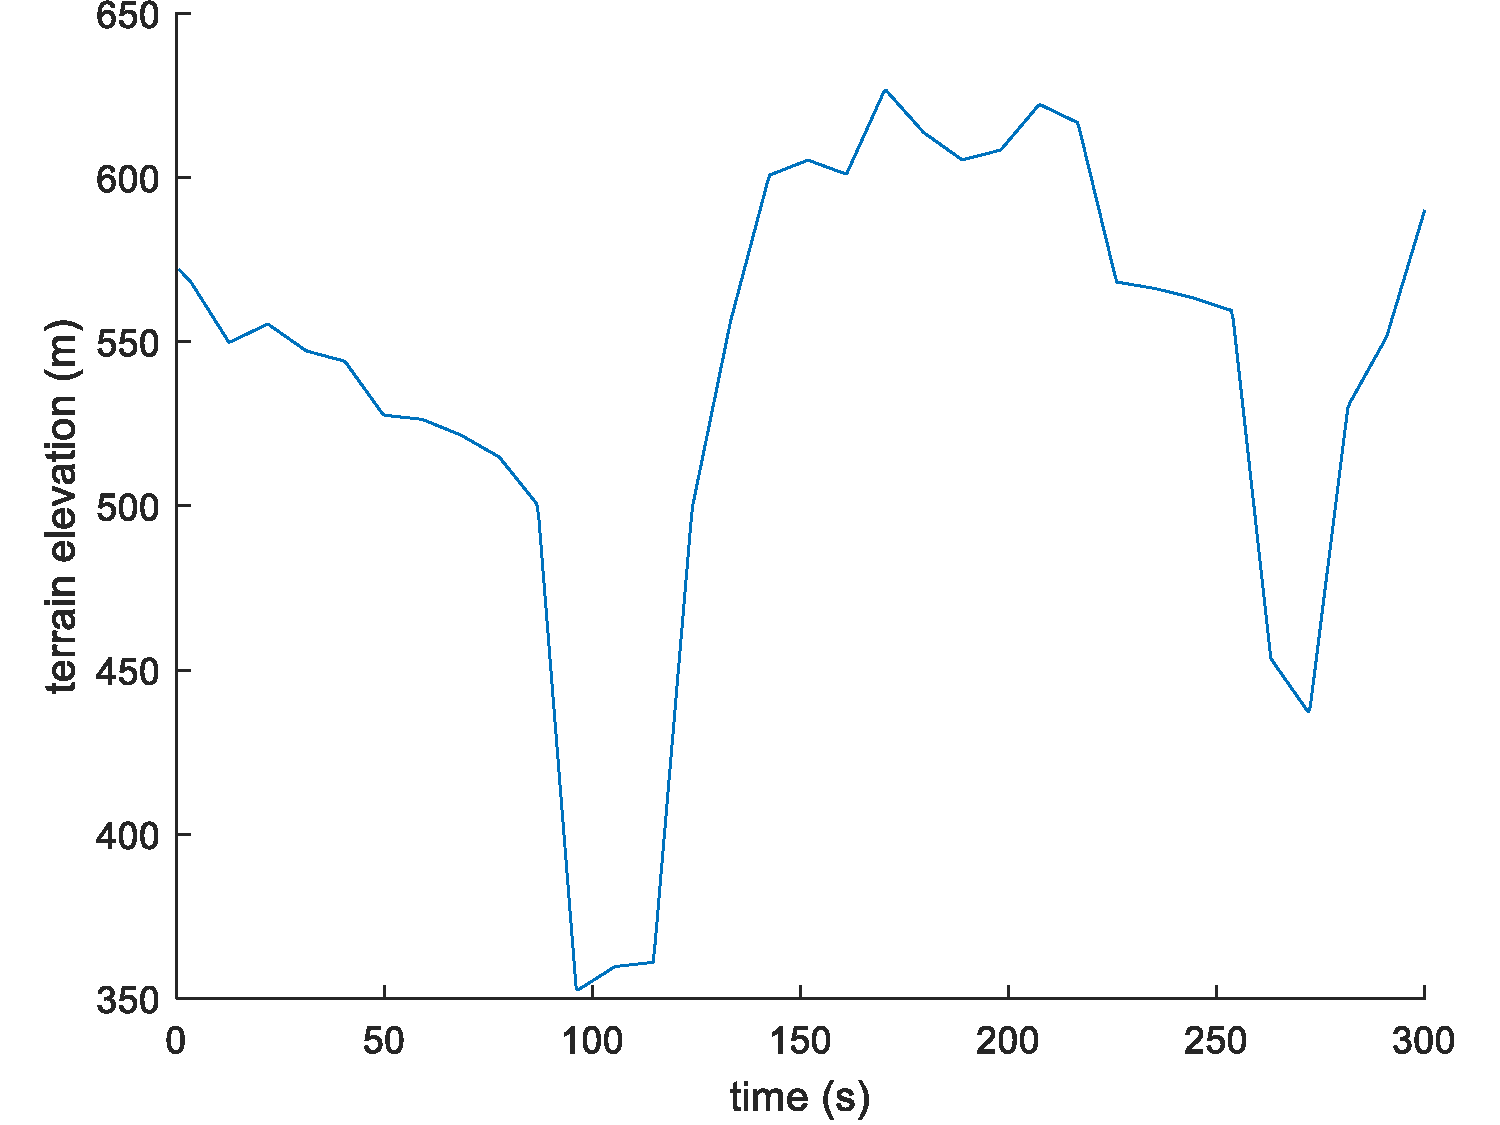
\includegraphics[width=6cm]{terrain.pdf}}
\caption{True terrain elevation under the UAV trajectory for each iteration of the navigation algorithm} \label{fig:terrain}
\end{figure}

The state is recursively estimated for $N_{iter}$ iterations by the AK-RPF, presented by Algorithm \ref{alg:AK-RPF}, from an estimation of the initial state $x_0$ of known covariance matrix $P_0$. The chosen resampling algorithm is the Kitagawa resampling. The mean function of the associated GP is assumed piecewise constant, and is equal to:
\begin{equation}
\mu : x \in \mathbb{R}^{d_x} \mapsto \frac{1}{\text{Card}(W_k)} \sum_{i \in W_k} \tilde z^i
\end{equation}

Its covariance function is a squared exponential:
\begin{equation}
k : (x, x') \in {\mathbb{R}^{d_x}}^2 \mapsto \sigma_f^2 \: \text{exp}\left(-\frac{1}{2} \frac{(x-x')^T (x-x')}{l^2}\right)
\end{equation}
and its hyperparameters are $\theta \triangleq [\sigma_f, \: l]^T$.

The sampled points are chosen to form a uniform mesh of the map, with resolution depending on $N_{GP}$. Table \ref{tab:parameters} presents the chosen value of the remaining parameters of the AK-RPF for this application.

\begin{table}[ht]
\renewcommand{\arraystretch}{1.3}
\centering \caption{Simulation and AK-RPF parameters} \label{tab:parameters}
\begin{tabular}{rl} \hline
Simulation & Value \\ \hline
$N_{iter}$ & $600$ \\
$\Delta_t$ & $0.5$ s \\
map surface & $40 \times 100$ km$^2$ \\
$P_0$ & $\text{diag}([2000, 2000, 100, 2, 2, 1])^2$ SI \footnotemark \\
$Q_k$ & $\text{diag}([40 ,40 ,2 ,0.4 ,0.4, .05])^2$ SI \\
$R_k$ & $15^2$ m$^2$ \\
$N_{GP}$ & $\in \{20^2, 30^2, \cdots, 80^2\}$ \\
$\tilde R$ & $15^2$ m$^2$ \\ \hhline{==}
AK-RPF & Value \\ \hline
$N_p$ & $5000$ \\
$\alpha_{th}$ & $0.5$ \\
$\alpha_{reg}$ & $0.3$ \\
$N_{W,min}$ & $10$ \\
$\alpha_W$ & $2$ \\
\hline
\end{tabular}
\end{table}
\footnotetext{{International System of Units, variance of positions in m$^2$, and of velocities in m$^2$s$^{-2}$}.}

\subsection{Numerical Results}

\begin{table*}[ht]
\renewcommand{\arraystretch}{1.3}
\centering \caption{Convergence rate, final RMSE and ARMSE for the RPF and AK-RPF at resolutions ranging between 0.40km and 3.50km} \label{tab:CV RMSE}
\begin{tabular}{|c|c|c|c|c|c|c|c|} \hline
\multirow{2}{*}{Resolution} & Number of & \multicolumn{3}{|c|}{RPF} & \multicolumn{3}{|c|}{AK-RPF} \\ \cline{3-8}
& points or $N_{GP}$ & Convergence & final RMSE & ARMSE & Convergence & final RMSE & ARMSE \\ \hlinewd{1.2pt}
0.40km & full map & 92\% & 0.97km & 1.99km & / & / & / \\ \hline
0.70km & $100^2$ & 34\% & 1.31km & 2.27km & / & / & / \\ \hline
0.78km & $90^2$ & 21\% & 1.61km & 2.60km & / & / & / \\ \hline
0.88km & $80^2$ & 3\% & 3.91km & 3.69km & 97\% & 0.43km & 1.16km \\ \hline
1.00km & $70^2$ & 0\% & N/A & N/A & 81\% & 1.08km & 1.82km \\ \hline
1.17km & $60^2$ & 0\% & N/A & N/A & 72\% & 1.15km & 2.17km \\ \hline
1.40km & $50^2$ & / & / & / & 55\% & 1.19km & 2.09km \\ \hline
1.75km & $40^2$ & / & / & / & 26\% & 2.35km & 2.61km \\ \hline
2.33km & $30^2$ & / & / & / & 1\% & 2.24km & 2.56km \\ \hline
3.50km & $20^2$ & / & / & / & 0\% & N/A & N/A \\ \hline
\end{tabular}
\end{table*}

Figure \ref{fig:navigation} shows a top view of a successful AK-RPF simulation for $N_{GP} = 80^2$. The true trajectory is in black, while the estimated trajectory is in red. The elevation map is given in the background according to the colormap on the right of the figure as an indication, and the kriging points are represented by black crosses. The position of each particle at the end of the simulation is shown in yellow, and the kriging window as well as the selected kriging data at the same time are respectively represented by red and black circles.

\begin{figure}[ht]
\centerline{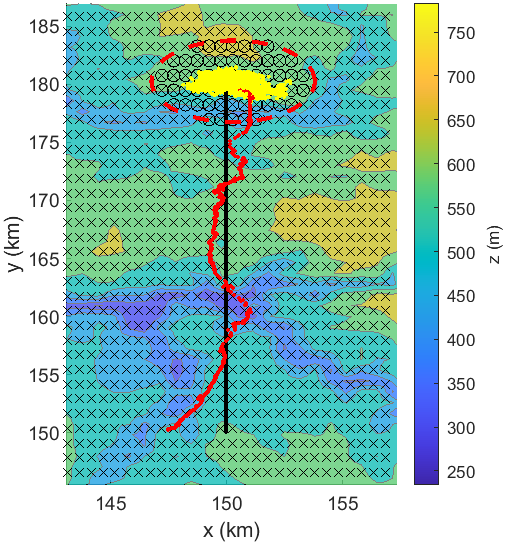
\includegraphics[width=6cm]{navigation.png}}
\caption{Visual output of the AK-RPF for a UAV TAN simulation using $N_{GP} = 80^2$ kriging points} \label{fig:navigation}
\end{figure}

For each possible value of $N_{GP}$, $100$ Monte Carlo runs were performed to evaluate the AK-RPF, and their convergence rate, final Root Mean Square Error (RMSE) and Average RMSE (ARMSE) were calculated. Comparisons with RPF using high-resolution and degraded maps were also performed. The degraded maps were reconstructed by performing bilinear interpolation on the same mesh used for kriging, and with the same noise, to ensure the validity of the comparison. The high-resolution map represents the ideal case, and has not been noised.

A run is considered convergent if the Mahalanobis distance between the estimate and the true state is inferior to a threshold for the last 5 iterations of the filter:
\begin{equation}
(x_k-\hat x_k)^T\:\hat P_k^{-1}\:(x_k-\hat x_k) < q^1_{1-99.73\%} \label{eq:CV criteria}
\end{equation}
where $q^1_{1-99.73\%}$ is the $99.73\%$ quantile of a $\chi^2_1$ distribution:
\begin{equation}
p(X\sim\chi^2_1 \leq q^1_{1-99.73\%})=99.73\%
\end{equation}

In the case of a Gaussian distribution, (\ref{eq:CV criteria}) means that the estimate remains within the $3\sigma$ confidence ellipsoid.

The convergence rate is defined as the ratio of the number of convergent runs to the total number of runs. The final RMSE and ARMSE are respectively defined as the value of the RMSE at the final iteration and its average over every iteration:
\begin{equation}
\text{final RMSE} \triangleq \text{RMSE}(N_{iter})
\end{equation}
\begin{equation}
\text{ARMSE} \triangleq \frac{1}{N_{iter}}\sum_{k=1}^{N_{iter}}\text{RMSE}(k)
\end{equation}
where the RMSE is:
\begin{equation}
\text{RMSE} : k \mapsto \sqrt{\frac{\sum_{mc\in E}||\varphi(x_k)-\varphi(\hat x_{k,mc})||_2^2}{\text{Card}(E)}}
\end{equation}
with $E$ the subset of convergent runs and $\varphi$ the orthogonal projector on the positions:
\begin{equation}
\varphi : x\text{ from (}\ref{eq:x}\text{)}\mapsto [p_x, \: p_y, \: p_z]^T
\end{equation}

Table \ref{tab:CV RMSE} presents the mentioned metrics for the tested bilinear RPFs and AK-RPFs. To help comparing the results, it also provides the resolution of the map or sampled data for each value of $N_{GP}$.

\begin{comment}
\begin{table}[ht]
\renewcommand{\arraystretch}{1.3}
\centering \caption{Convergence rate, final RMSE and ARMSE for the RPF and AK-RPFs for $N_{GP}$ varying between $20^2$ and $80^2$} \label{tab:CV RMSE}
\begin{tabular}{|c|c|c|c|} \hline
Filter & Convergence & final RMSE & ARMSE \\ \hline
RPF (known map) & 92\% & 0.97km & 1.99km \\ \hline
AK-RPF ($N_{GP}=20^2$) & 0\% & / & / \\ \hline
AK-RPF ($N_{GP}=30^2$) & 1\% & 2.24km & 2.56km \\ \hline
AK-RPF ($N_{GP}=40^2$) & 26\% & 2.35km & 2.61km \\ \hline
AK-RPF ($N_{GP}=50^2$) & 55\% & 1.19km & 2.09km \\ \hline
AK-RPF ($N_{GP}=60^2$) & 72\% & 1.15km & 2.17km \\ \hline
AK-RPF ($N_{GP}=70^2$) & 81\% & 1.08km & 1.82km \\ \hline
AK-RPF ($N_{GP}=80^2$) & 97\% & 0.43km & 1.16km \\ \hline
RPF ($70^2$ points) & 0\% & / & / \\ \hline
RPF ($80^2$ points) & 3\% & 3.91km & 3.69km \\ \hline
RPF ($90^2$ points) & 21\% & 1.61km & 2.60km \\ \hline
RPF ($100^2$ points) & 34\% & 1.31km & 2.27km \\ \hline
\end{tabular}
\end{table}

\begin{table}[ht]
\renewcommand{\arraystretch}{1.3}
\centering \caption{Correspondence between the number of points\\on the mesh and its resolution} \label{tab:resolutions}
\begin{tabular}{|c|c|c|c|c|} \cline{1-2}\cline{4-5}
Points & Resolution & & Points & Resolution \\ \cline{1-2}\cline{4-5}
known map & 0.40km & & $60^2$ & 1.17km \\ \cline{1-2}\cline{4-5}
$20^2$ & 3.50km & & $70^2$ & 1.00km \\ \cline{1-2}\cline{4-5}
$30^2$ & 2.33km & & $80^2$ & 0.88km \\ \cline{1-2}\cline{4-5}
$40^2$ & 1.75km & & $90^2$ & 0.78km \\ \cline{1-2}\cline{4-5}
$50^2$ & 1.40km & & $100^2$ & 0.70km  \\ \cline{1-2}\cline{4-5}
\end{tabular}
\end{table}
\end{comment}

Because the initial horizontal uncertainty is large ($2$km) and the overflown terrain is highly ambiguous (see Figure \ref{fig:terrain}), the process covariance matrix $Q_k$ has been chosen so that the particles explore a large area without losing diversity. This caused the final and average RMSEs shown on Table \ref{tab:CV RMSE} to remain elevated for every filter, even with the full non-degraded knowledge of the map.

On the other hand, the convergence rate steadily increases both for the AK-RPF and the bilinear RPF when given more prior information, and their associated RMSEs decrease accordingly, which means that the more information is given to the interpolation algorithm, the closer to truth it reconstructs the measurement function, and the better the filter estimates the state of the UAV.

However, the amount of information required for both filter is far from being similar. The AK-RPF is able to converge $72\%$ of the time with only $60^2$ points, which approximately corresponds to an under-sampling of $1$ noised kriging point for every $8.5$ points on the map, while the bilinear interpolation needs almost $3$ times as many points to reach half this convergent rate (which is an under-sampling of $1\!:\!3$). Similarly, the AK-RPF reaches the same final and average RMSE as the ideal case using $60^2$ kriging points, while the bilinear RPF is unable to reach this asymptote for the tested resolutions. This is because the bilinear interpolation is highly sensible to map noises, while the posterior mean function $\mu^*$ of the GP will smooth out sampling errors and give the precision of the interpolation to the filter in the form of the posterior covariance matrix $R^*$.

Figure \ref{fig:detail} shows in detail the evolution of the RMSE of 4 filters over the duration of the simulation: the fully-known map RPF, the $100^2$ points bilinear RPF, and the $N_{GP}=50^2$ and $N_{GP}=80^2$ AK-RPF.

\begin{figure}[ht]
\centerline{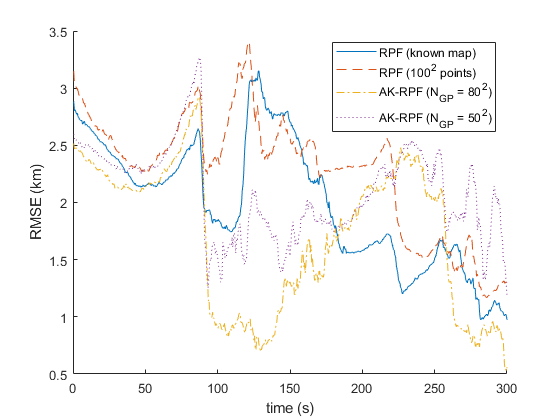
\includegraphics[width=8cm]{detail.png}}
\caption{Evolution of the RMSE over time for \mbox{RPF (known map)}, \mbox{RPF ($100^2$ points)}, AK-RPF ($N_{GP}=50^2$) and AK-RPF ($N_{GP}=80^2$)} \label{fig:detail}
\end{figure}

Figure \ref{fig:detail} further illustrates the kriging's ability to smooth the noised data to only retain relevant information for the measurement function, which alleviates ambiguities and reduces the risk of non-convergence. Indeed, the RMSE of both the AK-RPF ($N_{GP}=50^2$) and the AK-RPF ($N_{GP}=80^2$) drastically decreases when the UAV reaches the first pit (see Figures \ref{fig:terrain} and \ref{fig:navigation}) as this area yields a lot of information regarding the position of the UAV, and slowly increases again while it flies over an approximately flat, highly-ambiguous terrain. The RMSE then decreases again upon flying over the second pit for the same reason.

On the other hand, the highly noise-sensitive and extremely local interpolation (a bilinear interpolation uses the $4$ closest points, whereas kriging uses at least $N_{W,min} = 10$ points) performed by the RPF embedding a high-resolution map and the RPF ($100^2$ points) cannot grasp the trend surface of the map, and extracts less information from abrupt changes of terrain elevation than the kriging does. While the high-resolution map is not noisy, which allows its associate RPF to converge to the true state by using local variations to discriminate particles, the noise and the lack of resolution prevent the RPF ($100^2$ points) from doing the same.

\section{Conclusion and Future Work}
This paper focuses on solving the navigation problem in a poorly-known environment by reconstructing the measurement function solely based on scarce prior samples of the terrain. The innovation lies in the use of an adaptive-windowed Gaussian process combined with a regularised particle filter. This technique selects the most relevant prior data for regression at each iteration of the algorithm and dynamically estimates the hyperparameters of the Gaussian process by MLE. This new particle filter, called Adaptive Kriging Regularised Particle Filter (AK-RPF), has been applied to a TAN of UAV equipped with a radar altimeter. It outperforms the RPF based on classical bilinear interpolation methods by providing a more accurate and robust state estimation.

The main perspective to improving the AK-RPF is to use a Simultaneous Localisation And Mapping (SLAM) formalism by adding new data to the GPR during the mission. The Adaptive Kriging framework could also be extended to other types of Particle Filters.

\begin{thebibliography}{00}
\bibitem{bib:TAN1} C. Palmier, K. Dahia, N. Merlinge, P. Del Moral, D. Laneuville and C. Musso, "Adaptive Approximate Bayesian Computational Particle Filters for Underwater Terrain Aided Navigation". In: 2019 22th International Conference on Information Fusion (FUSION), pp. 1-8, 2019.

\bibitem{bib:TAN2} P.-J. Nordlund and F. Gustafsson, "Marginalized particle filter for accurate and reliable terrain-aided navigation”. In: IEEE Transactions on Aerospace and electronic systems, vol. 45, no. 4, pp. 1385–1399, 2009.

\bibitem{bib:TAN3} A. Murangira, C. Musso, K. Dahia, J.-M. Allard, "Robust regularized particle filter for terrain navigation". In: IEEE 14th International
Conference on Information Fusion, pp. 1-8, 2011.

\bibitem{bib:GP1} T. Imbiriba, J. C. M. Bermudez, J.-Y. Tourneret, C. Richard, "Detection of nonlinear mixtures using Gaussian processes: Application to hyperspectral imaging". In: 2014 IEEE International Conference on Acoustics, Speech and Signal Processing (ICASSP), pp. 7949-7953, 2014.

\bibitem{bib:GP2} T. Imbiriba, J. C. M. Bermudez, C. Richard, J.-Y. Tourneret, "Nonparametric detection of nonlinearly mixed pixels and endmember estimation in hyperspectral images", IEEE Transactions on Image
Processing, vol. 25, no. 3, pp. 1136-1151, 2016.

\bibitem{bib:GP3} P. I. Frazier, "A tutorial on Bayesian optimization", arXiv preprint, arXiv:1807.02811, 2018.

\bibitem{bib:Ristic} B. Ristic, S. Arulampalam and N. Gordon. "Beyond the Kalman filter: Particle filters for tracking applications". In: Artech house, 2003.

\bibitem{bib:RPF} C. Musso, N. Oudjane and F. Le Gland. "Improving regularized particle filters". In: Sequential Monte Carlo methods in practice, Springer, pp. 247-271, 2001.

\bibitem{bib:tutorial} M. S. Arulampalam, S. Maskell, N. Gordon and T. Clapp, "A tutorial on particle filters for online nonlinear/non-Gaussian Bayesian tracking". In: IEEE Transactions on Signal Processing, vol. 50, no. 2, pp. 174-188, Feb. 2002.

\bibitem{bib:weight variance} A. Doucet, S. Godsill and C. Andrieu, "On sequential Monte Carlo sampling methods for Bayesian filtering". In: Statistics and Computing, vol. 10, pp. 197-208, 2000.

\bibitem{bib:Epanechnikov} D. O. Loftsgaarden and C. P. Quesenberry, "A Nonparametric Estimate of a Multivariate Density Function''. In: The Annals of Mathematical Statistics, vol. 36, no. 3, pp. 1049-1051, Jun. 1965.

\bibitem{bib:Rasmussen} C. E. Rasmussen and C. K. I. Williams, "Gaussian Processes for Machine Learning". The MIT Press, 2006.
\end{thebibliography}

\end{document}
